\section{Solution Approach}

\subsection{Mixed-Integer Linear Program To Minimize Comms}

    % the full formulation of the milp

    The satellite-target custody problem can be solved used a mixed-integer linear program (MILP). 
    The performance parameters the system is trying to optimize is to minimize the communication costs of the system while also staying under computational limitations.
    In general, this type of satellite constellation is more limited by computation than communication, as there are many options for routing comms throughout neighboring nodes, but much harder constraints on the computational capacity of a satellite.
    Thus, the algorithm presented will set a hard constraint on the number of targets a fusion node can track, and then optimize to minimize communication costs to account for both the communication and computational performance.

    The MILP can be formulated as follows:

    \begin{equation}
        \underset{x_{st}}{\text{minimize}} \sum_{s} \sum_{t} c_{st} x_{st}
        \label{eq:objective}
    \end{equation}
    
    \text{subject to}

    \begin{equation}
        x_{st} \in \{0, 1\} 
        \label{eq:binary}
    \end{equation}

    \begin{equation}
        \sum_{s} x_{st} \geq 1 \quad \forall t
        \label{eq:constraint1}
    \end{equation}

    \begin{equation}
        \sum_{t} x_{st} \leq Comp(s) \quad \forall s
        \label{eq:constraint2}
    \end{equation}

    In the formulation above, $s$ is the index for a fusion satellite, and $t$ is the index for a target. \\
    Equation~\eqref{eq:objective} is the objective function, which is to minimize the cost of assigning custodies throughout the network (more dicussion on that cost below). \\
    Equation~\eqref{eq:binary} is the binary constraint, which ensures that the decision variable $x_{st}$ is either 0 or 1. If $x_{st} = 1$, then fusion satellite $s$ has custody of target $t$. \\
    Equation~\eqref{eq:constraint1} ensures that every target has at least one fusion satellite assigned to it. This means that each target is being tracked in the network. \\
    Equation~\eqref{eq:constraint2} ensures that no fusion satellite is assigned more targets than its computational limit, defined as $Comp(s)$. 

    The cost of assigning custody of a target to a fusion satellite is defined as $c_{st}$. A good cost function is one that minimizes the amount of communication throughout the network. 
    Since the goal of the algorithm is to assign custodies for some short horizon into the future, the cost function needs to account for current and future communication needs. 
    A simple choice for the cost function over some planning horizon $T$ is:
    \begin{equation}
        c_{st} = \sum_{k=0}^{T} \| \mathbf{r}_k^{target} - \mathbf{r}_k^s \|
        \label{eq:cost}
    \end{equation}

    The cost function is the sum of the distance between the estimated target position and the fusion satellite position over a discrete set of points from current time into the future horizon. 
    Future target position can be estimated by using the output of the track fusion algorithms. A extended kalman filter, as used in this paper, is able to output the estimated spherical dynamics of the targets, so this can be propagated forward in time to get an estimate of target position.
    Future satellite position is more easily known due to theconstant orbital parameters of a given satellite.
    This cost function is a good proxy for communication cost because it is a approximation for how far the measurement data needs to travel until it reaches the destination fusion satellite, thus, acting as a proxy for communication hops in the network. 
    By minimizing communication travel distance and number of hops, we are effectively minimizing the bandwidth usage and latency of the system.

\subsection{Overcapacity Case: Including Target Priority}

    % the full formulation of the milp with regional priority and how regional priority is included
    % also the modification 

     Although the above MILP is a good start, it does not account for scenarios where the number of targets requested to track is greater than the capacity of the system. 
     This is a very important edge case to consider and one that is often likely to happen in a real-world raid scenario.
     In a overcapacity case, the choice has to be made on which targets to track and which to not track. 
     Thus, the best way to solve this problem is to include notions of importance on the targets.

     To assign priority for targets, we will assume a priority is given to areas across the globe. Therefore, if a target is within that region, it is given the priority associated with that region.
     To implement priorities into the optimization problem, we will add a scaling factor, $f_{t}$, into the cost function which can account for this priority.
    
     \begin{equation}
        \underset{x_{st}}{\text{minimize}} \sum_{s} \sum_{t} c_{st} x_{st} \textcolor{red}{f_{t}}
        \label{eq:objective_priority}
    \end{equation}
    The priority factor function, $f_{t}$, can be defined as the following equation for a given target priority $p_{t}$:
    \begin{equation}
        f_{t} = X^{p_{t} - 1}
        \label{eq:exchange_rate}
    \end{equation}

    Equation~\eqref{eq:exchange_rate} is a good proxy to account for the impact of priorities on the cost function.
    The term $X$ is called the "exchange rate" and it's a constant that gives the relative importance of a priority level and the next priority level.
    I call it the exchange rate because it is the factor that scales the costs between priority levels.
    For example, if $X = 2$, then a target with priority 3 has 2 times the cost of a target with priority 2.
    Thus, a external user to the system can scale this exchange rate to give more or less weight to priorities, as desired.
    A graph showing the cost of varying priorities depending on the exchange rate is shown in Figure~\ref{fig:priority_cost}.
    
    \begin{figure}[h]
        \centering
        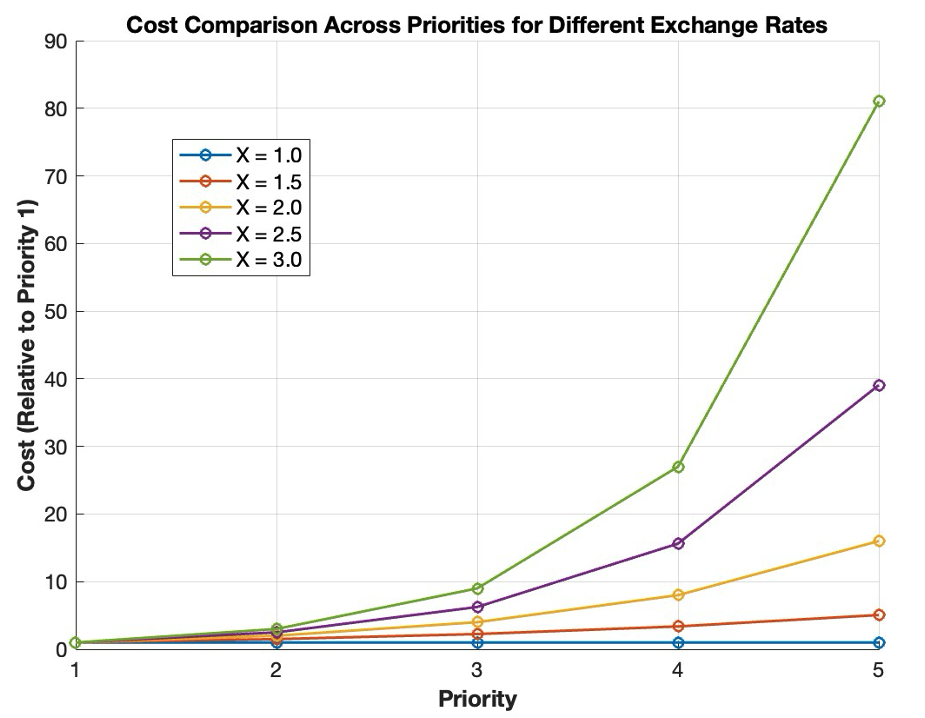
\includegraphics[width=0.5\textwidth]{figs/cost_vs_priority.png}
        \caption{Impact on exchange rate on the relative cost of priority levels}
        \label{fig:priority_cost}
    \end{figure}

    Additionally, the MILP needs to be modified to account for the overcapacity case.
    No longer, is the constraint given in Equation~\eqref{eq:constraint1} valid, as not every target can be tracked.
    Instead, the new constraint is given by:
    \begin{equation}
        \sum_{s} \sum_{t} x_{st} == \sum_{s} Capacity(s)
        \label{eq:constraint_overcapacity}
    \end{equation}

    Where $Capacity(s)$ is the computational capacity of the fusion satellite $s$. This new constraint ensures that the system is able to track as many targets as possible, fully saturating the satellites.

\subsection{Optimization Solver}

    %  talk about how used PuLP to solve the MILP, how pulp used branch and bound to solve the MILP

    The two MILP formulations presented above can be solved using off the shelf solvers. 
    Since the problem setup is in Python, as mentioned in the Problem Formulation section, a Python package called PuLP is used to solve the MILP \cite{b6}.
    PuLP is a Python package that is used to solve linear programming problems.
    This package uses the COIN-OR Branch and Cut Solver, which is a state-of-the-art solver for mixed-integer linear programs.
    This package uses open source mathmatical tools given by the Computational Infrastructure for Operations Research (COIN-OR) project \cite{b2}.  
    With these tools, the Branch and Cut algorithm is able to solve the MILP to global optimality, meaning that the solution is the optimal solution to the MILP.
    An example of how the Branch and Cut algorithm works is shown in Figure~\ref{fig:branch_and_cut}. 
    The algorithm works by first solving a linear program without the integer constraints using the Simplex algorithm \cite{b7}.
    Then, when a solution to the relaxed problem is obtained, a cutting plane algorithm is able to splice the solution by integer planes.
    This process is repeated until a solution is found that satisfies all constraints.

    \begin{figure}[h]
        \centering
        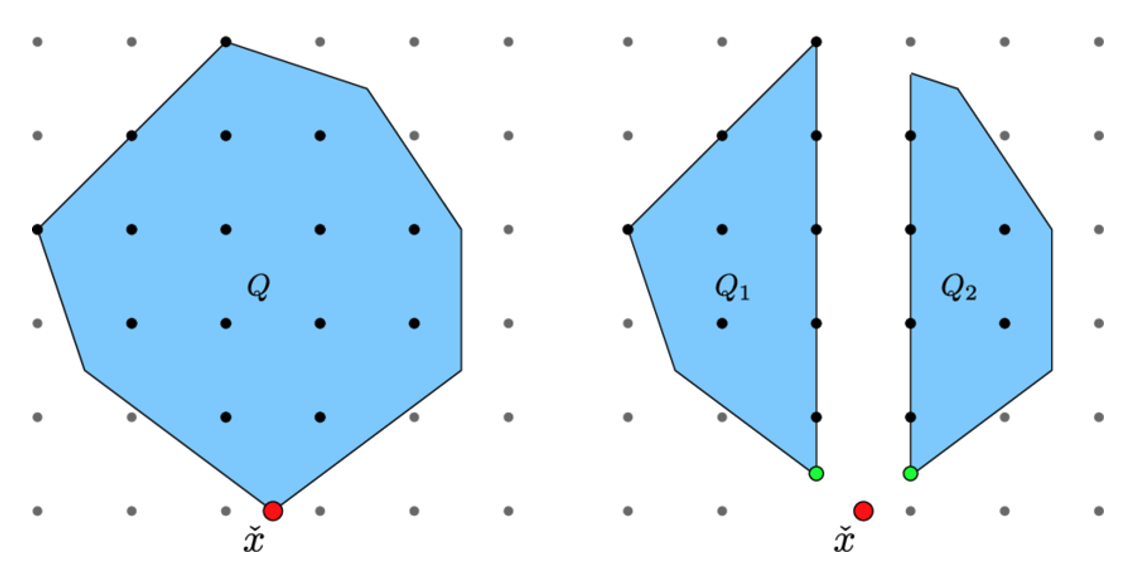
\includegraphics[width=0.45\textwidth]{figs/branch_and_cut.png}
        \caption{Branch and Cut Algorithm: cutting planes to get integer constraints}
        \label{fig:branch_and_cut}
    \end{figure}